\section{Capítulo 7 -- Vetores e matrizes}

Calcular a média de uma turma é fácil com um acumulador, como no Capítulo 5: cada nota é lida, somada e esquecida. Mas e se, depois da média, for preciso listar quem ficou acima dela? Agora as notas não podem ser esquecidas, porque cada uma vai ser comparada com um valor que só se conhece no fim. Declarar \texttt{nota1}, \texttt{nota2}, \ldots, \texttt{nota40} não resolve: o programa ficaria enorme e não serviria para uma turma de 41 alunos. A solução são as \textbf{estruturas de dados homogêneas}: o \textbf{vetor}, uma sequência de valores do mesmo tipo sob um único nome, e a \textbf{matriz}, uma tabela com linhas e colunas. Neste capítulo você vai aprender a declará-los, percorrê-los com laços, passá-los para funções e evitar o erro mais perigoso que eles trazem: acessar uma posição que não existe.

\subsection{7.1 O que é um vetor}

Um \textbf{vetor} (ou \textit{array}) é um conjunto de variáveis do mesmo tipo, guardadas lado a lado na memória e identificadas por um único nome. Cada variável do conjunto é um \textbf{elemento}, e é acessada pelo seu \textbf{índice}, a posição que ocupa no vetor, escrito entre colchetes: \texttt{notas[2]} é o elemento de índice 2 do vetor \texttt{notas}.

\begin{center}
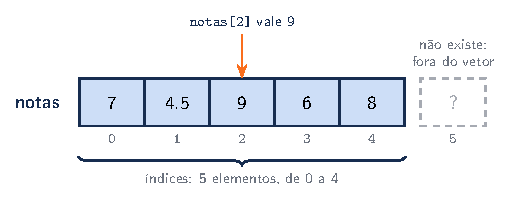
\includegraphics[width=0.8\linewidth,keepaspectratio]{imagens/capitulo-07_vetor.pdf}
\end{center}

Em C++, o primeiro índice é sempre \textbf{0}. Por isso, um vetor de 5 elementos tem os índices de 0 a 4, e o último elemento de um vetor de tamanho \texttt{n} é o de índice \texttt{n - 1}. Na declaração, o número entre colchetes é o \textbf{tamanho}, que precisa ser uma constante:

\begin{codigo}
\begin{Verbatim}[breaklines=true, breaksymbolleft={}, fontsize=\footnotesize]
#include <iostream>
using namespace std;

int main() {
    double notas[5];                  // 5 elementos, de 0 a 4
    notas[0] = 7;
    notas[1] = 4.5;
    notas[4] = notas[0] + 1;          // 8

    int primos[] = {2, 3, 5, 7, 11};  // tamanho deduzido: 5
    int contagem[10] = {};            // todos começam em 0
    int i = 3;
    cout << primos[i] << " " << primos[i + 1] << endl;   // 7 11
    cout << notas[4] << " " << contagem[9] << endl;      // 8 0
    return 0;
}
\end{Verbatim}
\end{codigo}

Como uma variável comum, um vetor declarado sem valores iniciais contém lixo. A lista entre chaves preenche os elementos na ordem, e os que sobram ficam com 0: por isso \texttt{= \{\}} é a forma mais curta de zerar um vetor inteiro. O índice pode ser qualquer expressão inteira, como \texttt{i} ou \texttt{i + 1}, e é isso que torna o vetor poderoso: um laço pode visitar todos os elementos mudando apenas o índice.

\subsection{7.2 Percorrendo um vetor com laços}

O \texttt{for} e o vetor foram feitos um para o outro: o contador do laço serve de índice e passa por todas as posições, da primeira à última. O programa abaixo resolve o problema do início do capítulo. O primeiro laço lê as notas e as soma; o segundo, que só pode ser feito depois que a média é conhecida, mostra as que ficaram acima dela.

\begin{codigo}
\begin{Verbatim}[breaklines=true, breaksymbolleft={}, fontsize=\footnotesize]
#include <iostream>
using namespace std;

int main() {
    const int MAX = 50;
    double notas[MAX] = {};
    int n;
    cout << "Quantos alunos (até 50)? ";
    cin >> n;
    if (n < 1 || n > MAX) {
        cout << "Quantidade inválida." << endl;
        return 0;
    }
    double soma = 0;
    for (int i = 0; i < n; i++) {
        cout << "Nota " << i + 1 << ": ";
        cin >> notas[i];
        soma += notas[i];
    }
    double media = soma / n;
    cout << "Média: " << media << endl;
    cout << "Acima da média:";
    for (int i = 0; i < n; i++) {
        if (notas[i] > media) cout << " " << notas[i];
    }
    cout << endl;
    return 0;
}
// 4 alunos com 7, 4.5, 9 e 6 -> Média: 6.625
// Acima da média: 7 9
\end{Verbatim}
\end{codigo}

Repare em três detalhes. O vetor é declarado com uma capacidade máxima (\texttt{MAX}), porque seu tamanho precisa ser conhecido na compilação, e o programa usa só as \texttt{n} primeiras posições. O \texttt{if} logo depois da leitura garante que \texttt{n} cabe no vetor. E o laço vai de \texttt{0} enquanto \texttt{i < n}, a forma padrão de percorrer \texttt{n} elementos em C++; para o usuário, que conta a partir de 1, o programa mostra \texttt{i + 1}.

Em Portugol, o vetor é declarado com o tipo \texttt{vetor}, informando o primeiro e o último índice. Diferente do C++, quem escolhe os limites é o programador, e o mais comum é começar em 1:

\begin{codigo}
\begin{Verbatim}[breaklines=true, breaksymbolleft={}, fontsize=\footnotesize]
algoritmo "AcimaDaMedia"
var
   notas: vetor[1..50] de real
   n, i: inteiro
   soma, media: real
inicio
   escreva("Quantos alunos (até 50)? ")
   leia(n)
   soma <- 0
   para i de 1 ate n faca
      escreva("Nota ", i, ": ")
      leia(notas[i])
      soma <- soma + notas[i]
   fimpara
   media <- soma / n
   escreval("Média: ", media)
   escreval("Acima da média:")
   para i de 1 ate n faca
      se notas[i] > media entao
         escreval(notas[i])
      fimse
   fimpara
fimalgoritmo
\end{Verbatim}
\end{codigo}

\subsection{7.3 Cuidado com os limites}

O que acontece com \texttt{notas[5]} em um vetor de 5 elementos? Em C++, a resposta é: \textbf{qualquer coisa}. A linguagem não confere se o índice existe. Ela simplesmente calcula onde estaria o elemento 5, logo depois do último, e lê ou escreve naquela posição da memória, que pertence a outra variável ou nem pertence ao programa.

\begin{codigo}
\begin{Verbatim}[breaklines=true, breaksymbolleft={}, fontsize=\footnotesize]
// erro: índices fora do vetor
int v[5] = {1, 2, 3, 4, 5};
for (int i = 0; i <= 5; i++) {   // <= faz uma volta a mais
    cout << v[i] << " ";         // v[5] não existe
}
v[-1] = 0;                       // nem v[-1]
\end{Verbatim}
\end{codigo}

O resultado é chamado de \textbf{comportamento indefinido}: o programa pode mostrar um valor sem sentido, alterar silenciosamente outra variável, travar ou, o pior caso, funcionar normalmente nos testes e falhar mais tarde. O compilador às vezes avisa quando o índice é uma constante, mas nunca quando ele vem de um cálculo. Esse tipo de erro, conhecido como \textbf{estouro de vetor} (\textit{buffer overflow}), já foi a porta de entrada de muitos ataques a sistemas, porque permite escrever onde o programa não deveria.

A defesa é disciplina: percorra com \texttt{i < n}, e não \texttt{i <= n}; confira, antes de usar, todo índice que vem do usuário ou de um cálculo; e nunca deixe o número de elementos passar da capacidade declarada. O Portugol do VisuAlg, ao contrário do C++, interrompe a execução com uma mensagem de erro quando o índice sai dos limites.

\subsection{7.4 Algoritmos clássicos com vetores}

\subsubsection{Contagem por categoria}

Quando os valores possíveis são poucos números inteiros, o próprio valor pode servir de índice. O programa abaixo apura uma pesquisa de satisfação com notas de 1 a 5: em vez de cinco contadores separados, um vetor \texttt{votos}, em que \texttt{votos[k]} conta quantas vezes a nota \texttt{k} apareceu.

\begin{codigo}
\begin{Verbatim}[breaklines=true, breaksymbolleft={}, fontsize=\footnotesize]
#include <iostream>
#include <string>
using namespace std;

int main() {
    int votos[6] = {};        // usa 1 a 5; a posição 0 sobra
    int voto;
    cout << "Notas de 1 a 5 (0 para terminar): ";
    while (cin >> voto && voto != 0) {
        if (voto >= 1 && voto <= 5) {
            votos[voto]++;    // o voto é o índice
        }
    }
    for (int k = 1; k <= 5; k++) {
        cout << k << ": " << string(votos[k], '*')
             << " (" << votos[k] << ")" << endl;
    }
    return 0;
}
\end{Verbatim}
\end{codigo}

Com a entrada \texttt{5 4 5 3 5 4 1 0}, a saída é um pequeno gráfico de barras, desenhado com \texttt{string(n, \textquotesingle{}*\textquotesingle{})}, que cria um texto com \texttt{n} asteriscos:

\begin{codigo}
\begin{Verbatim}[breaklines=true, breaksymbolleft={}, fontsize=\footnotesize]
// saída
1: * (1)
2:  (0)
3: * (1)
4: ** (2)
5: *** (3)
\end{Verbatim}
\end{codigo}

O \texttt{if} que confere a faixa é essencial: sem ele, um voto 9 escreveria em \texttt{votos[9]}, fora do vetor.

\subsubsection{Maior elemento e sua posição}

O padrão do maior valor, do Capítulo 5, ganha uma informação extra com vetores: \textbf{onde} o maior está. Basta guardar o índice em vez do valor, começando pelo primeiro elemento:

\begin{codigo}
\begin{Verbatim}[breaklines=true, breaksymbolleft={}, fontsize=\footnotesize]
#include <iostream>
using namespace std;

int main() {
    double temp[7] = {22.5, 25.1, 27.8, 24.0, 28.3, 26.6, 21.9};
    int iMaior = 0;                  // começa pelo primeiro
    for (int i = 1; i < 7; i++) {
        if (temp[i] > temp[iMaior]) iMaior = i;
    }
    cout << "Dia mais quente: " << iMaior + 1
         << " (" << temp[iMaior] << " graus)" << endl;
    return 0;                        // dia 5 (28.3 graus)
}
\end{Verbatim}
\end{codigo}

\subsubsection{Invertendo um vetor}

Para inverter um vetor no próprio lugar, troca-se o primeiro com o último, o segundo com o penúltimo, e assim por diante, com dois índices que caminham um em direção ao outro até se encontrarem no meio:

\begin{codigo}
\begin{Verbatim}[breaklines=true, breaksymbolleft={}, fontsize=\footnotesize]
#include <iostream>
using namespace std;

int main() {
    int v[6] = {1, 2, 3, 4, 5, 6};
    for (int i = 0, j = 5; i < j; i++, j--) {
        int aux = v[i];              // a troca do Capítulo 6
        v[i] = v[j];
        v[j] = aux;
    }
    for (int i = 0; i < 6; i++) cout << v[i] << " ";
    cout << endl;                    // 6 5 4 3 2 1
    return 0;
}
\end{Verbatim}
\end{codigo}

A condição \texttt{i < j} é o ponto delicado: com \texttt{i < 6}, o laço inverteria o vetor e depois o desinverteria, voltando ao original. A biblioteca do C++ oferece a função \texttt{swap(v[i], v[j])}, que faz a mesma troca das três linhas. Outros algoritmos clássicos com vetores, a busca de um valor e a ordenação, têm um capítulo inteiro, o 10.

\subsection{7.5 Vetores e funções}

Um vetor pode ser passado para uma função, com uma diferença importante em relação às variáveis comuns: ele \textbf{não é copiado}. A função recebe a localização do vetor original na memória, e por isso tudo o que ela altera nos elementos fica alterado para quem chamou, como na passagem por referência. Além disso, a função não tem como descobrir o tamanho do vetor: ele precisa ser passado em um parâmetro separado.

\begin{codigo}
\begin{Verbatim}[breaklines=true, breaksymbolleft={}, fontsize=\footnotesize]
#include <iostream>
using namespace std;

double media(const double v[], int n) {   // const: só lê
    double soma = 0;
    for (int i = 0; i < n; i++) soma += v[i];
    return soma / n;
}

void aumentar(double v[], int n, double bonus) {
    for (int i = 0; i < n; i++) {
        v[i] += bonus;
        if (v[i] > 10) v[i] = 10;        // nota máxima: 10
    }
}

int main() {
    double notas[4] = {7, 4.5, 9.8, 6};
    cout << "Antes: " << media(notas, 4) << endl;   // 6.825
    aumentar(notas, 4, 0.5);             // altera o original
    cout << "Depois: " << media(notas, 4) << endl;  // 7.25
    return 0;
}
\end{Verbatim}
\end{codigo}

O parâmetro é escrito com colchetes vazios, \texttt{double v[]}. Quando a função só lê o vetor, como \texttt{media}, o \texttt{const} documenta isso e faz o compilador recusar qualquer alteração por engano. Uma função também não pode devolver um vetor com \texttt{return}: para produzir um vetor, ela recebe um vetor de quem chama e o preenche.

No VisuAlg, vetores não podem ser passados como parâmetro. Os subprogramas trabalham com o vetor declarado na seção \texttt{var} do algoritmo, que é global, e recebem por parâmetro apenas os valores simples, como a quantidade de elementos.

\subsection{7.6 Matrizes}

Muitos dados têm duas dimensões: as notas de cada aluno em cada prova, as vendas de cada loja em cada mês, os pixels de uma imagem, o tabuleiro de um jogo. Para eles existe a \textbf{matriz}, um vetor de duas dimensões, em que cada elemento é identificado por dois índices: a \textbf{linha} e a \textbf{coluna}.

\begin{center}
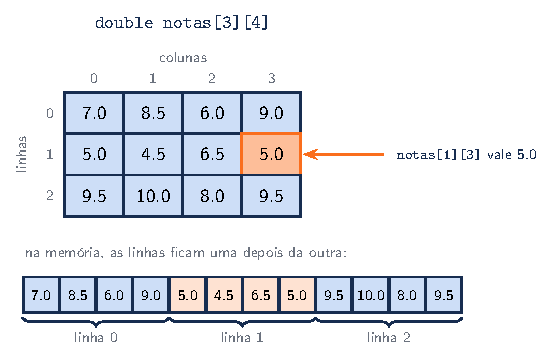
\includegraphics[width=0.85\linewidth,keepaspectratio]{imagens/capitulo-07_matriz.pdf}
\end{center}

Em C++, a matriz é declarada com dois tamanhos, \texttt{double notas[3][4]} (3 linhas e 4 colunas), e cada elemento é acessado com dois pares de colchetes: \texttt{notas[1][2]} é o elemento da linha 1, coluna 2. Na memória, as linhas ficam uma depois da outra, como mostra a parte de baixo da figura.

Percorrer uma matriz pede dois laços aninhados (Capítulo 5): o de fora passa pelas linhas e, para cada linha, o de dentro passa pelas colunas. O programa abaixo calcula a média de cada aluno (somando uma linha) e a média de cada prova (somando uma coluna):

\begin{codigo}
\begin{Verbatim}[breaklines=true, breaksymbolleft={}, fontsize=\footnotesize]
#include <iostream>
using namespace std;

const int ALUNOS = 3, PROVAS = 4;

int main() {
    double notas[ALUNOS][PROVAS] = {
        {7.0, 8.5, 6.0, 9.0},       // aluno 0
        {5.0, 4.5, 6.5, 5.0},       // aluno 1
        {9.5, 10.0, 8.0, 9.5}       // aluno 2
    };
    for (int i = 0; i < ALUNOS; i++) {          // cada linha
        double soma = 0;
        for (int j = 0; j < PROVAS; j++) soma += notas[i][j];
        cout << "Aluno " << i + 1 << ": " << soma / PROVAS
             << endl;
    }
    for (int j = 0; j < PROVAS; j++) {          // cada coluna
        double soma = 0;
        for (int i = 0; i < ALUNOS; i++) soma += notas[i][j];
        cout << "Prova " << j + 1 << ": " << soma / ALUNOS
             << endl;
    }
    return 0;
}
// Aluno 1: 7.625   Aluno 2: 5.25   Aluno 3: 9.25
// Prova 1: 7.16667   Prova 2: 7.66667 ...
\end{Verbatim}
\end{codigo}

Compare os dois pares de laços: para somar uma \textbf{linha}, a linha \texttt{i} fica fixa e a coluna \texttt{j} varia; para somar uma \textbf{coluna}, é o contrário. Trocar os papéis de \texttt{i} e \texttt{j} é um dos erros mais comuns com matrizes.

Em Portugol, a matriz também é um \texttt{vetor}, declarado com os limites das duas dimensões separados por vírgula, e os dois índices também vão separados por vírgula:

\begin{codigo}
\begin{Verbatim}[breaklines=true, breaksymbolleft={}, fontsize=\footnotesize]
algoritmo "NotasDaTurma"
var
   notas: vetor[1..3, 1..4] de real
   i, j: inteiro
   soma: real
inicio
   para i de 1 ate 3 faca
      soma <- 0
      para j de 1 ate 4 faca
         escreva("Aluno ", i, ", prova ", j, ": ")
         leia(notas[i, j])
         soma <- soma + notas[i, j]
      fimpara
      escreval("Média do aluno ", i, ": ", soma / 4)
   fimpara
fimalgoritmo
\end{Verbatim}
\end{codigo}

Para passar uma matriz a uma função em C++, o número de \textbf{colunas} precisa aparecer no parâmetro, como em \texttt{void mostrar(const double m[][PROVAS], int linhas)}. Só o número de linhas pode ficar vazio, porque o compilador precisa saber o tamanho de cada linha para calcular onde começa a linha seguinte.

\subsection{7.7 Um programa completo: jogo da velha}

O tabuleiro do jogo da velha é uma matriz $3 \times 3$ de caracteres. Para saber se alguém venceu, é preciso verificar as 3 linhas, as 3 colunas e as 2 diagonais. Na \textbf{diagonal principal}, a linha e a coluna são iguais (\texttt{t[0][0]}, \texttt{t[1][1]}, \texttt{t[2][2]}); na \textbf{diagonal secundária}, elas somam 2 (\texttt{t[0][2]}, \texttt{t[1][1]}, \texttt{t[2][0]}).

\begin{codigo}
\begin{Verbatim}[breaklines=true, breaksymbolleft={}, fontsize=\footnotesize]
#include <iostream>
using namespace std;

bool iguais(char a, char b, char c) {
    return a != ' ' && a == b && b == c;   // casa vazia não vale
}

char vencedor(const char t[3][3]) {
    for (int i = 0; i < 3; i++) {
        if (iguais(t[i][0], t[i][1], t[i][2])) return t[i][0];
        if (iguais(t[0][i], t[1][i], t[2][i])) return t[0][i];
    }
    if (iguais(t[0][0], t[1][1], t[2][2])) return t[1][1];
    if (iguais(t[0][2], t[1][1], t[2][0])) return t[1][1];
    return ' ';                            // ninguém venceu
}

void mostrar(const char t[3][3]) {
    for (int i = 0; i < 3; i++) {
        cout << " " << t[i][0] << " | " << t[i][1]
             << " | " << t[i][2] << endl;
        if (i < 2) cout << "---+---+---" << endl;
    }
}

int main() {
    char t[3][3] = {
        {'X', 'O', 'X'},
        {'O', 'X', 'O'},
        {' ', 'O', 'X'}
    };
    mostrar(t);
    char v = vencedor(t);
    if (v == ' ') cout << "Ninguém venceu ainda." << endl;
    else cout << "Venceu: " << v << endl;   // Venceu: X
    return 0;
}
\end{Verbatim}
\end{codigo}

O laço de \texttt{vencedor} aproveita a mesma variável \texttt{i} para as linhas (\texttt{t[i][...]}) e para as colunas (\texttt{t[...][i]}). A função \texttt{iguais} evita repetir a mesma comparação oito vezes e, ao exigir \texttt{a != \textquotesingle{} \textquotesingle{}}, impede que uma linha vazia seja contada como vitória. Para testar, monte tabuleiros que vençam por linha, por coluna, por cada diagonal, e um sem vencedor.

\subsection{7.8 Vetores com tamanho variável: vector}

O vetor da linguagem C++, herdado da linguagem C, tem tamanho fixo e não confere índices. A biblioteca padrão oferece uma alternativa mais segura e flexível, o \texttt{vector}, que cresce conforme os elementos são acrescentados e sabe o próprio tamanho:

\begin{codigo}
\begin{Verbatim}[breaklines=true, breaksymbolleft={}, fontsize=\footnotesize]
#include <iostream>
#include <vector>
using namespace std;

int main() {
    vector<double> notas;            // começa vazio
    double nota;
    cout << "Notas (negativo para terminar): ";
    while (cin >> nota && nota >= 0) {
        notas.push_back(nota);       // acrescenta no fim
    }
    double soma = 0;
    for (size_t i = 0; i < notas.size(); i++) soma += notas[i];
    if (!notas.empty()) {
        cout << notas.size() << " notas, média "
             << soma / notas.size() << endl;
    }
    return 0;
}
// Entrada: 7 4.5 9 6 -1  ->  4 notas, média 6.625
\end{Verbatim}
\end{codigo}

Com \texttt{vector}, não é preciso definir uma capacidade máxima nem guardar a quantidade em outra variável: \texttt{push\_back} acrescenta um elemento e \texttt{size()} informa quantos há. O tipo \texttt{size\_t}, um inteiro sem sinal, é o tipo de \texttt{size()}, e usá-lo no contador evita um aviso do compilador. O acesso com \texttt{notas[i]} continua sem conferência, mas \texttt{notas.at(i)} confere o índice e interrompe o programa com uma mensagem de erro se ele não existir. Nos capítulos seguintes, sempre que o tamanho não for conhecido de antemão, o \texttt{vector} será a escolha natural.

\subsection{Erros Comuns}

\begin{itemize}
  \item \textbf{Começar ou terminar no índice errado.} Em C++, os índices vão de 0 a \texttt{n - 1}. Percorra com \texttt{for (int i = 0; i < n; i++)}.
  \item \textbf{Acessar fora dos limites.} \texttt{v[n]}, \texttt{v[-1]} ou um índice vindo do usuário sem conferência levam a comportamento indefinido.
  \item \textbf{Esquecer de inicializar.} Um vetor de contadores precisa começar zerado: \texttt{int votos[6] = \{\};}.
  \item \textbf{Usar mais elementos do que a capacidade.} Confira se a quantidade lida cabe no vetor antes do laço de leitura.
  \item \textbf{Achar que a função recebe uma cópia do vetor.} Ela trabalha no original. Use \texttt{const} quando a função só deve ler.
  \item \textbf{Esquecer de passar o tamanho para a função.} Dentro dela, não há como descobri-lo.
  \item \textbf{Trocar linha e coluna.} Em \texttt{m[i][j]}, o primeiro índice é a linha. Para somar uma linha, fixe \texttt{i}; para somar uma coluna, fixe \texttt{j}.
  \item \textbf{Escrever \texttt{m[i, j]} em C++.} Essa é a sintaxe do Portugol. Em C++, são dois pares de colchetes: \texttt{m[i][j]}.
\end{itemize}
